%-----------------------------------------------------------------------------%
%Packages%
\documentclass[12pt, a4paper, titlepage]{article}
\usepackage{amsmath, amsfonts, listings, amssymb, mathtools, amsthm} %Mathematical Expressions package
\usepackage{mathtools}
\usepackage[usenames, dvipsnames]{color} %Color naming packages
\usepackage{geometry}
\usepackage{float}
\usepackage{verbatim} %for code
\usepackage[pdftex]{graphics}
\usepackage{hyperref}
\usepackage{cleveref}
\usepackage{tikz}
\usepackage[nottoc]{tocbibind}
\usepackage{caption}
%\usepackage{subcaption}
\usepackage{fancyhdr}

\usetikzlibrary{arrows,shapes}

%Graphis Extensions
\DeclareGraphicsExtensions{.png, .jpg}
\parindent 0pt

% Predefined things such as commands, etc.
\newcommand{\FIXME}{{\bf FIXME}}
\newcommand{\major}{{\bf major }}
\newcommand{\minor}{{\bf minor }}
\newcommand{\easy}{{\bf easy }}
\newcommand{\hard}{{\bf hard }}
% Drawings of frames

\tikzstyle{vertex}=[circle,fill=black!25,minimum size=20pt,inner sep=0pt]
\tikzstyle{selected vertex} = [vertex, fill=red!24]
\tikzstyle{edge} = [draw,thick,->]
\tikzstyle{weight} = [font=\small]

\setlength{\headheight}{15.2pt}
\pagestyle{fancy}

\fancyhf[FC]{\thepage}
\fancyhf[HL]{Edwin Richard Yucheng Tay, 20529864}
\fancyhf[HR]{CITS5502 Assignment Two}

%-----------------------------------------------------------------------------%
%Document%

\title{CITS5502: Assignment Two}
\author{Edwin Richard Yucheng Tay \\
University of Western Australia \\
email: taye03@student.uwa.edu.au }

\date{\today}

\begin{document}

\maketitle

\tableofcontents

\section{Introduction --- TODO by 0930 14th August 2013} \label{introduction}

In today's software development industry, the methodology of software development is fractured
between multiple processes.
Some companies use an ``agile" methodology, iteratively developing ideas and prototyping their
products \FIXME. %need a citation
Others develop according to the traditional Software Development Lifecycle (SDLC) models, requiring
extensive documentation and requirements before beginning software development \FIXME.\\
\\
These are confusing categorisations, and within each are further sub-models, such as \FIXME
%citations below
\begin{itemize}
	\item ``Spiral"
	\item ``Extreme Programming"
	\item ``Prototyping"
	\item ``V-Model"
\end{itemize}
Depending on what project, some development processes are not even suitable for some software
projects and it is thus desirable to gauge how suitable one process is compared to another.\\
\\
However, each is denoted in its own format and style, making identification and classification of processes a
confusing task \FIXME. %add diagrams
Comparisons about the strengths and weaknesses of each process and their suitability to fulfill a
project are thus difficult to conceive.\\
\\
We will resolve these difficulties in by introducing a simple flow-chart based notation with some
relations to UML-activity diagrams.
This standardised notation will be further augmented with a descriptive aid and translation to a
C-style imperative language.\\
\\
We construct a taxonomy based on the distinguishing features between a set of software development
processes.
Our taxonomy will have two aims
\begin{enumerate}
	\item given a software development process, which known software development process does it most
	resemble?
	\item given a description of informal software requirements, which known software development
	process would be suitable for its development?
\end{enumerate}

Finally, we present an analysis of the taxonomy and significant or interesting results we have
found during through the taxonomy.
We discuss what makes our taxonomy and classification system worthwhile for usage and present
conjectures about improving classification methods.

\section{Constraints --- TODO by 30 August 2013}

\FIXME Fluff text

Modelling is the field of formalising assumptions about the world in logical and mathematical terms.
The formality of such models allows us to test, validate and analyse our model using objective, rather than subjective observations.
However, the more assumptions we make, the more specific our model is.
Perhaps it even makes our model less useful, because it is too specific.
Conversely, the less assumptions we make, the more general our model is.
But implicitly, it is more difficult to model (as there are more variables to capture).\\
\\
As we are building a (formal) model for defect detection and fixing, it is implicit that we too will make assumptions that we encode into our model.
It is thus worthwhile to discuss our observations and assumptions.
More importantly, we ought to justify why assumptions could be made and what their impact on the results are.\\
\\
This chapter begins by describing our problem, in terms of observations and open questions.
We then lay down our assumptions to answer the open questions, as well as justifications for {\em why} these assumptions were made.
We summarise our results in our final subchapter.

\subsection{Observations}

We will lay down our model assumptions by first describing the data we are working with.
We are given data about a two-stage process which finds, then fixes defects.
This project involves 3 software engineers who worked 25 hours per week, where one engineer was testing.
The data provided is the result of that engineer devoting all of his/her time to testing each
week and uncovering defects.\\
\\
Defects can be classed into 2 levels of ``severity", and 2 levels of "difficulty".
They are of either \major or \minor severity, and either \easy or \hard in terms of difficulty.
We are told that \major defects are approximately ``seven times as damaging on average as minor
ones".
Furthermore, on average a \hard defect requires 5 hours to fix, whilst an \easy defect requires 2
hours to fix \FIXME.
We shall take on the role of the project manager and use models to simulate different strategies against different
metrics.\\
\\
This describes the data and initial constraints of our model.
There are many open questions that we ought to at least consider, and hopefully answer before
beginning our modelling.
We enumerate them below
\begin{enumerate}
	\item can an engineer do ``part of" a defect?
	For example, if an engineer has 1 hour left in their working week, can they do half of an \easy
defect? \label{openQuestOne}
	\item we have estimated the ``impact" --- how does this translate to impacting the customer?
	Is it by money?
	By time?
	Should we assign some units to it, or is the arbitrary ``severity" measure good enough?
	\label{openQuestTwo}
	\item are our estimates of ``severity" and ``difficulty" accurate?
	If they are not, how accurate are they actually, and how does inaccuracy translate in our model?
	\label{openQuestThree}
	\item when do defects get fixed?
	In real life, the defect detection/fixing process is a two-stage parallel process, where detection
puts defects onto an ordered priority queue of defects to fix, whilst fixing simultaneously takes
defects from the priority queue for fixing.
	This is illustrated in Figure \ref{realDefectProcess}. \label{openQuestFour}
	\item does the testing engineer only do testing?
	Can they do other work?
	Are they as effective at doing other work? \label{openQuestFive}
	\item if a testing engineer can do other work, when do they stop testing and start other work?
	And when do they become a testing engineer again? these questions apply equally to a normal software engineer and we ought to answer them for
the development engineers \label{openQuestSix}. 
	\item when a defect is fixed, does it reintroduce bugs or is it always fixed?
	\label{openQuestEight}
	\item if we had twice as many testers, would we go through our defect detection data twice as
quickly? \label{openQuestNine}
	\item does a defect only affect the customers the moment the tester has found them?
	Indeed, is the tester the only way of a defect to be detected? \label{openQuestTen}
	\item what do we actually want to measure? \label{openQuestEleven}
\end{enumerate}

\begin{figure}
	\FIXME the defect detect/fix process
	\caption{derp} \label{realDefectProcess}
\end{figure}

We will now outline and justify our assumptions, and answer the open questions we have raised as
best we can.

\subsection{Assumptions about our simulation}

Firstly, Question \ref{openQuestOne} asks whether we can have ``part fixes".
We will disallow this in our simulation --- it makes the model more realisitc but at this stage it
is too difficult to model.
For Question \ref{openQuestTwo} we will simply let the model measure severity in its
unitless form --- there is less to be gained from attaching some unit to it since we have no concept
of what our client values and how they are being affected here.\\
\\
For Question \ref{openQuestThree}, we are going to assume the estimates are exactly accurate.
This is, of course, a blatant falsehood --- there are estimation techniques such as \FIXME which
indicate the {\em confidence} of an estimate.
Indeed, estimates are seemingly useless without some idea of standard deviation or variance.
Nevertheless, for ease of modelling we will let the values for \easy, \hard, \minor and \major be
exact values of the difficulty and severity of fixing a defect.\\
\\
Question \ref{openQuestFour} again opens a method by which the accuracy of our model, and its power
could be much improved.
If the defect fixing and detection process actually resembles Figure \ref{realDefectProcess}, our
model would be quite an accurate representation of the real world.
This is difficult to actually build into our model, however.
For the purposes of this paper, we limit our model to a sequential, instead of parallel defect
detection and fixing process.
This process is shown in Figure \ref{fakeDefectProcess}

\begin{figure}[ht!]
	\FIXME the defect detect/fix process
	\caption{derp} \label{fakeDefectProcess}
\end{figure}

Questions \ref{openQuestFive} and \ref{openQuestSix} ask whether a software engineer should be reassigned from testing, and
when that should occur.
We will allow this, and its occurrance is something we are interested in.
How should we allocate resources?
When should we do so?
These are artefacts of the strategies we use, and the simulation will allow a strategy to test
this.
We will also say that all software engineers are equally competent at testing and development,
although it is true, according to \FIXME that some engineers might be approximately twenty times
more skilled than another engineer.\\
\\
We say for Question \ref{openQuestEight} that a defect will not reintroduce bugs into our system.
For Question \ref{openQuestNine} we claim that this is indeed the case, and if we assign more people
to testing then the effect scales multiplicatively.
Conversely, the fewer people in testing, the slower defect detection will be.
People also cannot split their time between defect detection and defect fixing --- they are either
doing one or the other the whole time.
Of course, all of this is not an accurate reflection of the real world (indeed, Brooks espouses in
\FIXME why the assumption of more people speeding up software work is particularly flawed), but again
it eases the modelling process.\\
\\
Finally, we say that for Question \ref{openQuestTen}, the only person finding defects are the
testers.
Implicitly, a developer can only fix a defect after a tester has found it.\\

\subsection{What are we measuring?}

To answer Question \ref{openQuestEleven}, we must also give thought to 
\begin{itemize}
	\item what we are measuring
	\item assumptions about how the client behaves and
	\item what interests both us and them.
\end{itemize}

To begin with, let us discuss the tangential topic of ``internal" and ``external"
perspectives on a project.
\FIXME notes that a software engineering project has two views --- the ``internal" view, which is
that of a software organision, and the ``external" view, which is that of a client.
We want to be able to model our process in terms of these metrics, to gauge the client's view of our
efforts, and also make useful measurements for our own ``internal" usage.
Note that this does {\em not} mean that an ``external" metric is not useful for the ``internal"
metrics --- rather, we say that ``internal" metrics measure things that are less desired or useful
to the client than an ``external" metric.\\
\\
We will make the following assumptions about the client behaviour
\begin{itemize}
	\item clients prefer major defects to be fixed over minor defects --- this seems logical since a
client is being affected negatively seven times more by a major defect, than by a minor one
	\item clients prefer defects to be fixed quickly --- this is evidenced by \FIXME
\end{itemize}

We will aim to measure the following ``external" metrics
\begin{itemize}
	\item queue severity --- a simple sum that takes into the total importance of found defects yet to
be fixed.
	Note that it does not increase the severity for defects that have been in the queue for longer ---
according to \FIXME this degrades client satisfaction and it was actually an oversight of my
modelling process to not do this.
	\item on average, how long have major defects been within the queue?
	This is related to our above comments on the importance of timeliness of fixes and the perception
that slow fixes has on clients, as shown in \FIXME
	\item the estimated number of major defects remaining in the system, an important estimate to a
client
\end{itemize}

We will also measure the following ``internal" metrics
\begin{itemize}
	\item the estimated number of defects remaining, no matter what severity or difficulty they are
--- this will give us a stopping criteria.
	We will assume that an exponential line of best fit can be fitted to the data, using a model
similar to Boehm's COCOMO equations \FIXME.
	We thus expect that the number of defects remaining in a system can be modelled by a negative
exponential, as in Figure \ref{negExp}.
	\item the size of our defect queue --- indeed, this is a metric that could be used in an audit,
though whether such a measurement is appopriate for an audit of our processes or teams is another
unrelated matter
	\item the average time a defect has been in our defect queue
	\item the ratio of defects fixed to defects found in that week
	\item the ratio of major defects to major defects found in that week
\end{itemize}

\begin{figure}[ht!]
	\caption{Neg exp \FIXME} \label{negExp}
\end{figure}

\subsection{Summary of metrics and assumptions}

In summary, we make the following assumptions:
\begin{itemize}
	\item no partial fixes
	\item unitless severity
	\item all estimates are reliable and entirely accurate
	\item sequential, as opposed to parallelised defect fixing process
	\item engineers can be reassigned --- an artefact of the strategy
	\item engineers are all equally competent
	\item defect fixing does not reintroduce defects
	\item having $k$ testers implies we will complete our work $k$ times as quickly
	\item only the tester is finding the defects, and developers cannot fix a defect unless a tester
has found it
\end{itemize}

These assumptions seem, perhaps, to be very trivial or to not reflect the actual state of a software
engineering project.
The observant reader will note that the reasons for most of these assumptions are ``they make the modelling
process easier".
It is unfortunate that these notions cannot at this stage be challeneged, but we will give a
treatise later on how we might challenge or improve our models.\\
\\
We will measure the following ``external" metrics
\begin{itemize}
	\item queue severity
	\item the average amount of time, in weeks, that a major defect is in the queue
	\item the estimated number of major defects remaining in the system
\end{itemize}

We will also measure the following ``internal" metrics.
\begin{itemize}
	\item the estimated number of defects remaining
	\item the size of our defect queue
	\item the average time, in weeks, that a defect has been in our defect queue
	\item the ratio of defects fixed to defects found in that week
	\item the ratio of major defects to major defects found in that week
\end{itemize}

\section{Measurements}

This is the main bulk of our paper, and we discuss the method with which we approached this problem,
the strategies we implemented and our results.

\subsection{Methodology}

To model this system, we constructed a simulation framework in C++.
This framework translated and encoded our assumptions as best as we could.
It used basic C++ polymorphism to capture the ideas of Metrics, Strategies and Simulations and then
write them to files.\\
\\
A more complete description of its inner workings is described in Appendix \ref{simframe}.
We will review the strengths and weaknesses of this approach in the analysis, found in Section
\ref{analysis}.

\subsection{Strategies}

We will look at three strategies for defect detection and fixing.
In particular, we will also vary these strategies according to some metrics, and say that a
simulation is finished according to the results of another metric.\\
\\
Firstly, we make the following assumptions about a strategy for defect detection and fixing.
\begin{itemize}
	\item a strategy is stateful in the sense that it remembers previous defect detections and makes
judgements on whether to finish or to reallocate resources based on that state
	\item since it is stateful, strategies are inherently measuring and then making decisions based on
a metric and it is thus reasonable to assume that strategies require metrics to function well
	\item a strategy should at all times allocate all engineers to some task
	\item a strategy will reorder the defect queue based upon some criterion of the strategy
	\item strategies will favour defects found earlier over defects found later
	\item strategies will stop when a system is estimated to have too few defects remaining or the
number of defects has stabilised to the point that it is a waste of resources to continue testing
\end{itemize}

We will look at the following three strategies
\begin{enumerate}
	\item first-in-first-out (FIFO) --- earlier defects are favoured over later defects, but there is no
ordering between these defects.\\
	As an example, all defects in week 1 will be placed ahead in the queue compared to defects found
in week 2, but the hard, easy, major and minor defects of week 1 have no inherent ordering over each
other
	\item easy first --- extends the FIFO strategy, by now placing an ordering that we prefer easy
defects to hard defects, and then major defects to minor defects.\\
	This means that, in order, we prefer easy major defects, then easy minor defects, then hard major
defects, and lastly hard minor defects.\\
	\item major first --- extends the FIFO strategy, by now placing an ordering that we prefer major 
defects to minor defects, and then easy defects to hard defects.\\
	This means that, in order, we prefer easy major defects, then hard major defects, then easy minor 
defects, and lastly hard minor defects.\\
\end{enumerate}

Our variations on these strategies will be simple resource reallocations, based on either internal
or external pressure.
\begin{itemize}
	\item no variation --- the strategy runs as prescribed and no resource changes occur
	\item external pressure --- the client is being heavily affected by the defects, so the tester is
temporarily reallocated to defect fixing
	\item internal pressure --- upper-level management is unimpressed by the size of the defect queue,
so a tester is temporarily reallocated to defect fixing
\end{itemize}

The actual, well-defined points for when management or a client becomes dissatisfied are somewhat
arbitrarily chosen.
We will expand upon this more within the experiments section, and our later analysis.
We feel that this arbitrariness is a good reflection of real life, however.

Other strategies that we could look at, but will discard are
\begin{itemize}
	\item solve the defects in a random order --- this is illogical, and as our models are supposed to
somewhat reflect real life processes, why should we do something that is entirely contrived and has
no basis in the real world whatsoever?
	\item solve te hard defects first --- this has the least gains for our internal metrics, and a greedy approach dictates
that this is the least efficient use of our time.
	Why solve defects that take more time and are less impactful for the user (and also give us bad
performance overall) when we can pick solve easier problems?
	\item solve minor defects first -- again this has few gains, from the user point of view, since
high impact problems that are really affecting productivity are being ignored.
	If this leads to client dissatisfaction, then why use this strategy?
\end{itemize}

\subsection{Experiments}

We display the results of our experiments in graphical form, and finally make comments and tabulate
which strategies showed the most promising results.

\subsubsection{No change of resources}

We first begin by looking at the external metrics.
This governs what the client (might!) be thinking about our project and the strategies we have used.

\begin{figure}[ht!]
	\centering
	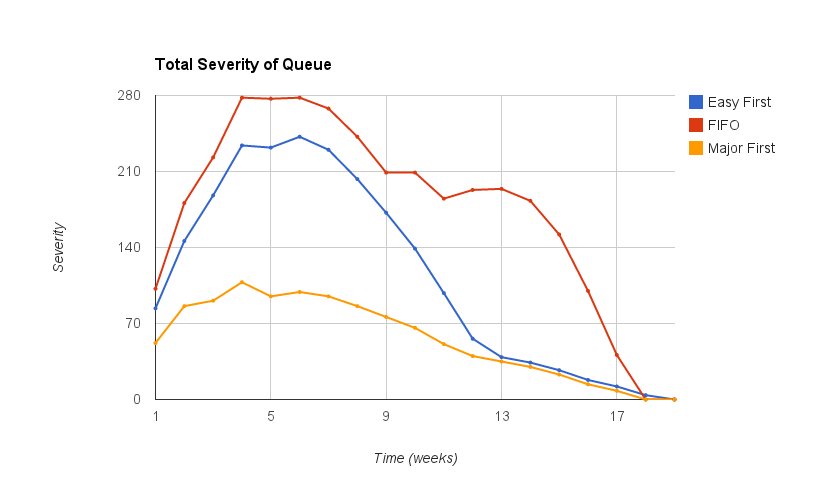
\includegraphics[scale=0.5]{graphs/QueueImpact.png}
	\caption{The severity of the defects yet to be fixed is shown here.
Of note is that defects perhaps should be more impactful the longer they are left in the queue ---
but are we then measuring reputation, money or productivity?
Beyond this, it is quite clear that at this stage fixing major defects first is a good strategy to
take, as it consistently keeps the queue impact low by fixing lots of major defects.} 
	\label{qimpact}
\end{figure}

It is clear that fixing major defects is the best choice according to this metric.
What about the average time of major defects in the queue?
This gives us an idea of how long users have been waiting for a fix to a critical error.

\begin{figure}[ht!]
	\centering
	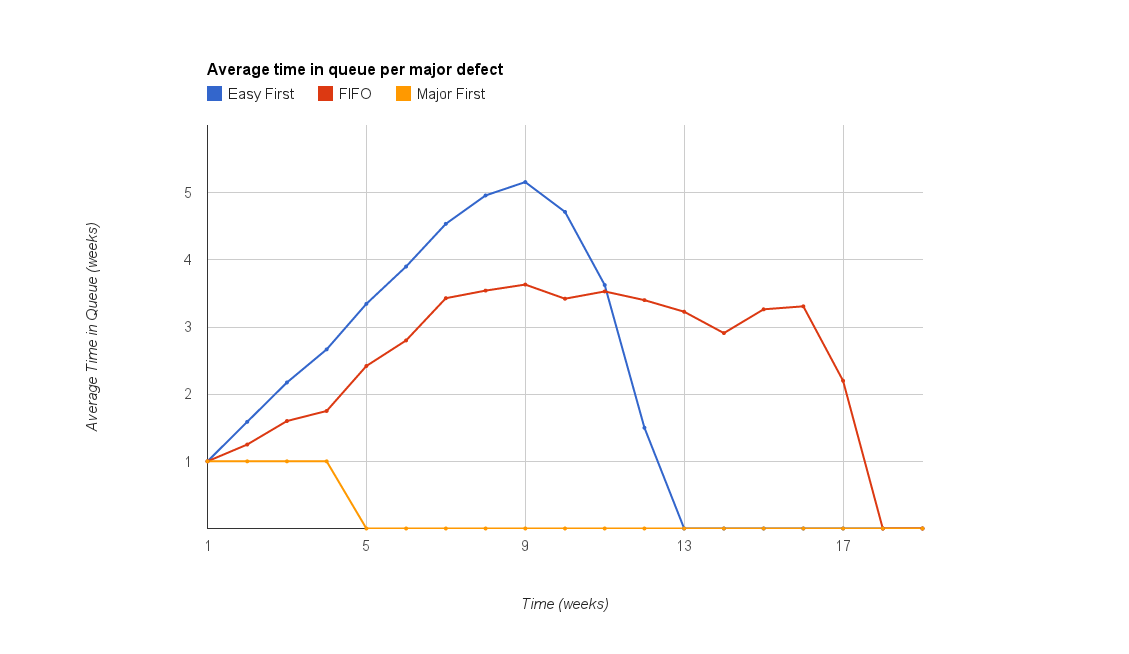
\includegraphics[scale=0.45]{graphs/avgMajorQueueTime.png}
	\caption{High prioritisation of major defects is very helpful here!
	We see that major defects are being fixed almost as they come arrive in the major strategy, whilst
the FIFO and easy-first strategies allow the time in queue to blow up to high values.} 
	\label{avgmajqtime}
\end{figure}

From Figure \ref{avgmajqtime} it is clear that fixing major defects is the best choice to have a
high performance for average major queue time.
This is inherently due to the focus on major defects and giving the customer what they are
interested in (or so we presume).\\
\\
Next, we briefly examine the find-versus-fixed ratio for major defects.

\pagebreak

\begin{figure}[ht!]
	\centering
	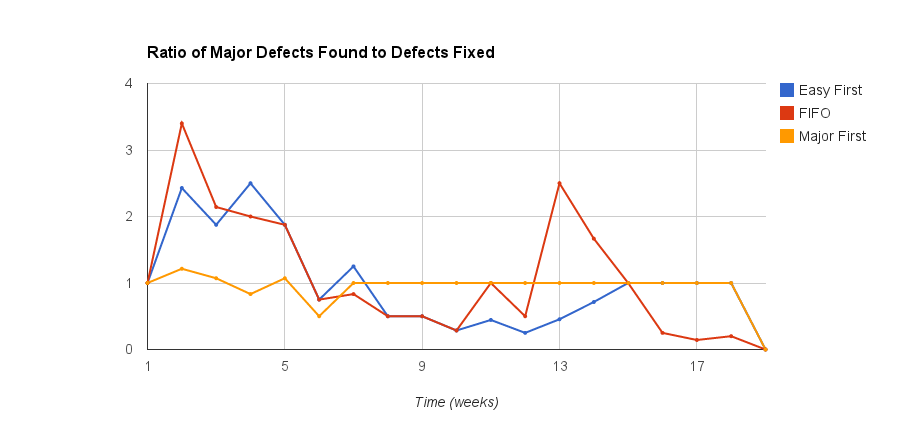
\includegraphics[scale=0.45]{graphs/MajRatioFF.png}
	\caption{High prioritisation of major defects is very helpful here!
	We see that major defects are being fixed almost as they come arrive in the major strategy, whilst
the FIFO and easy-first strategies allow the time in queue to blow up to high values.} 
	\label{majratioff}
\end{figure}

Again we see that the optimal strategy for this metric is to fix major defects first --- not very
surprising!
But it is interesting to note that here, the differences are not so great --- especially towards the
end, the major-fixes-first are either on par or even suboptimal compared to the other two
strategies.\\
\\
Finally in Figure \ref{estremmajdef}, we examine the estimation of how many major defects remain in the system.

\pagebreak

\begin{figure}[ht!]
	\centering
	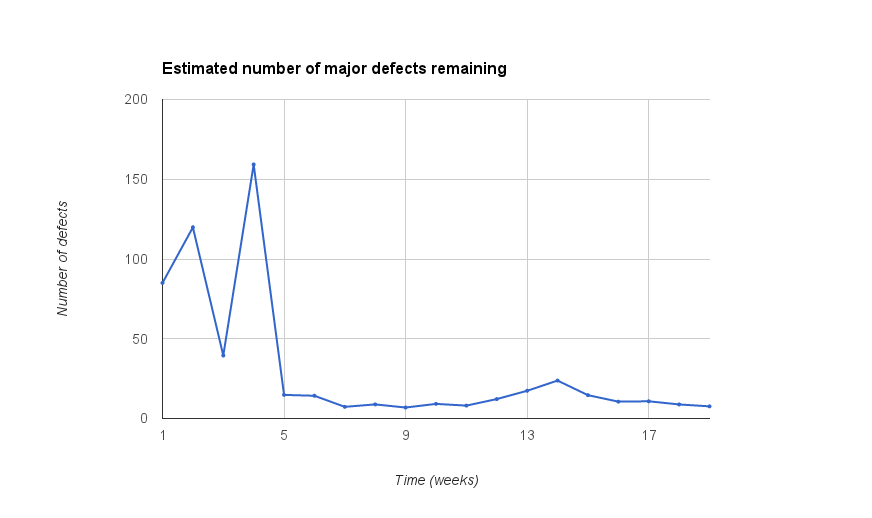
\includegraphics[scale=0.5]{graphs/EstRemMajDef.png}
	\caption{Since each defect has the same detection policies, each of them had the same curve and
there is no ``better" detection here.} 
	\label{estremmajdef}
\end{figure}

It is clear that towards the end of the process there are very few major defects remaining.
But why stop there?\\
\\
To answer this question, we now show the results of our internal metrics.
We begin with the metric ``how many defects do we estimate remain in our system?"

\pagebreak

\begin{figure}[ht!]
	\centering
	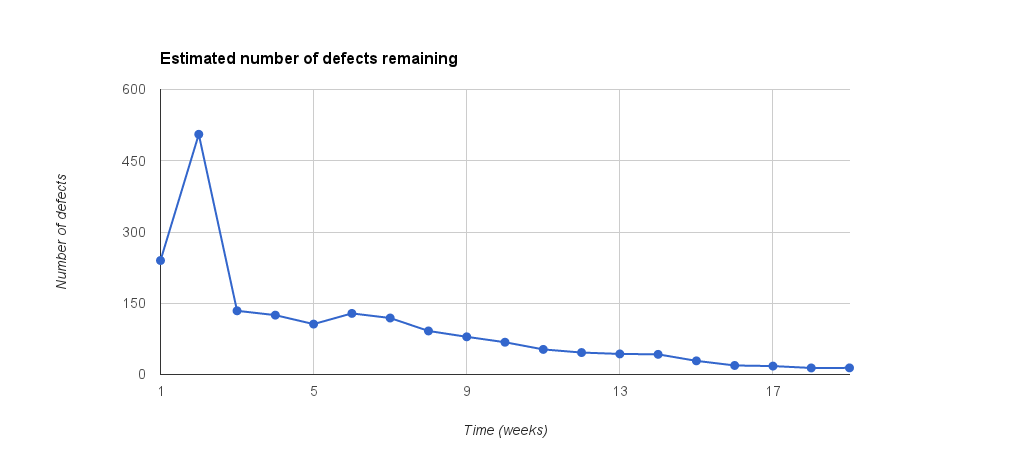
\includegraphics[scale=0.45]{graphs/EstRemDefs.png}
	\caption{Notice how few defects there are towards the end. This is part of the criteria for
stopping a simulation, and the strategy decided that further testing was a waste of resources due to
the estimate saying that the defect counting had stabilised.} 
	\label{estremdefs}
\end{figure}

Again, the system stability and low number of estimated defects towards the end of the development
process is an indicator as to why a project manager would say the project is completed.
But how good are the strategies at keeping the number of defects that need to be fixed low?

\pagebreak

\begin{figure}[ht!]
	\centering
	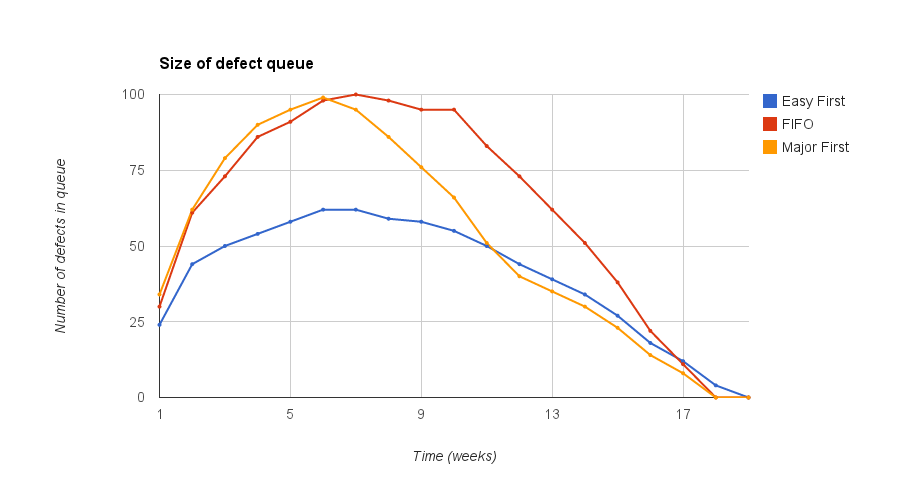
\includegraphics[scale=0.45]{graphs/QueueSz.png}
	\caption{The size of our defects-to-fix queue. The seemingly optimal choice is to use the easy
strategy.} 
	\label{qsz}
\end{figure}

Figure \ref{qsz} gives what would be the self-evident result --- that prioritising easy defects
yields the best rewards.
This is simply because taking easy defects first results in the highest number of defects being
fixed and the queue size shrinking fastest.\\
\\
We would expect something similar to occur when looking at the average time a defect spends in a
queue, wouldn't we?

\pagebreak

\begin{figure}[ht!]
	\centering
	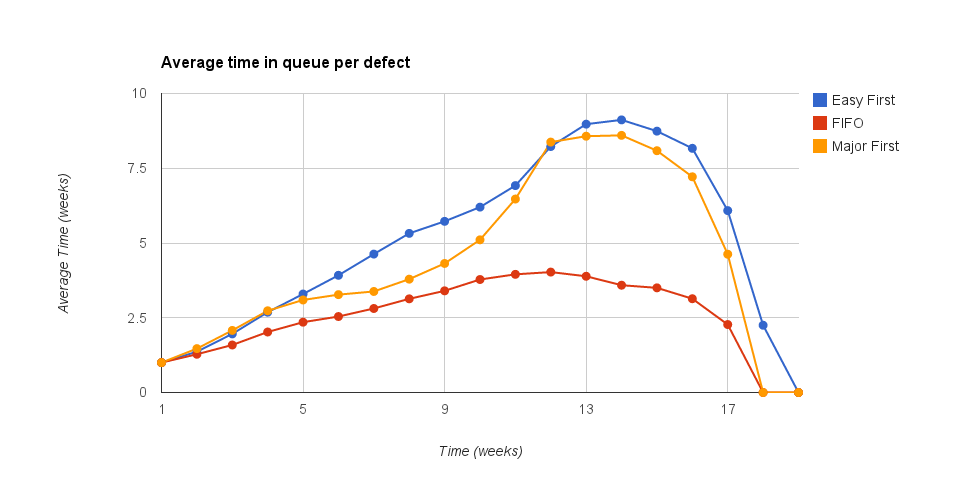
\includegraphics[scale=0.45]{graphs/avgQueueTime.png}
	\caption{The average time a defect spends in the queue is of course actually minimsed by the FIFO
strategy, since it endeavours to fix earliest defects as soon as possible, without any other
reorderings.} 
	\label{avgqtime}
\end{figure}

This does not really go against our logic --- it is a proof that at least without resource
reallocations the system behaves as we expect.\\
\\
Finally, we showcase the defect ratios for find-versus-fixed.

\pagebreak

\begin{figure}[ht!]
	\centering
	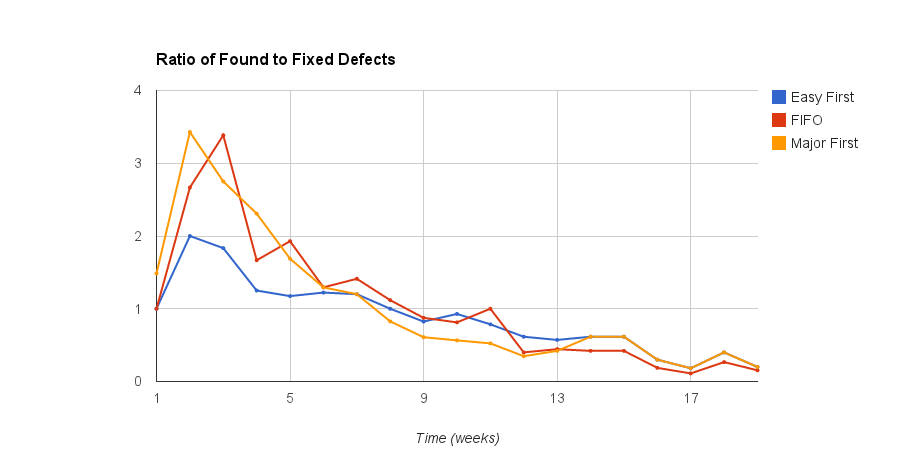
\includegraphics[scale=0.5]{graphs/RatioFF.png}
	\caption{Here, we notice that the optimal choice is to use the easy strategy again, which is a
reflection of our previous metrics and how the easy strategy fixes the highest number of defects.} 
	\label{ratioff}
\end{figure}

As expected, Figure \ref{ratioff} shows that the easy strategy is the optimal for performance using
this metric.\\
\\
We have tabulated our results in a coarse approximation of how ``good" each strategy performed for
each metric.

\begin{table}[ht!]
	\centering
	\begin{tabular}{|c|c|c|}
	\hline
	{\bf Metric} & {\bf Optimal} & {\bf Sub-optimal, but close?} \\ \hline
	{\em Queue Severity} & Major First & N/A \\ \hline
	{\em Mean time in queue per major defect} & Major First & N/A\\ \hline
	{\em Ratio of Major defects found-to-fixed} & Major First & Easy-first \\ \hline
	Queue Size & Easy First & N/A \\ \hline
	Time in Queue & FIFO & Not that close, but Major First \\ \hline
	Ratio of defects found-to-fixed & Easy First & Major First\\ \hline
	\end{tabular}
	\caption{A summary of our strategies and their performances with different metrics.
External metrics are italicised.
It seems clear that the strategy which externally appears best is major first, whilst internally
easy-first appears best.}
	\label{summary}
\end{table}

\subsubsection{External pressure leading to resource change}

Now, we suppose that if the queue severity is too high (that is, existing defects are negatively
affecting the client too much) then a resource reallocation is required.
It is not a very intelligent decision making system, in that it simply reallocates the resources for
the week and keeps them allocated as such until the queue severity is low again.
We can compare it to a bang-bang controller in embedded systems and robotics.\\
\\
Before we begin, we will note an experimental error that we came across but were too late in fixing.
During our measurements for estimating the number of defects left, the FIFO strategy had some
strange occurrences and started outputting negative estimates.
We could not trace where the error in our methodology is, and we have removed it from our
comparisons for external influences.
We present the initial estimates with FIFO included to show how the results were mangled.

\begin{figure}[ht!]
	\centering
	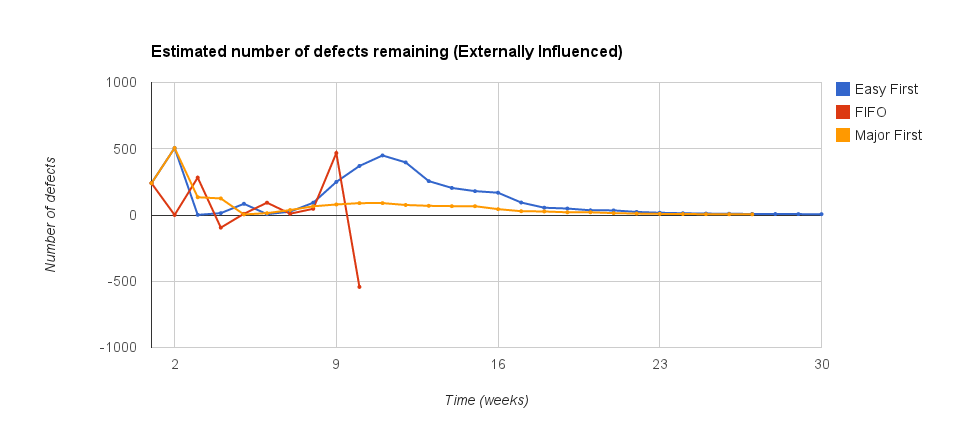
\includegraphics[scale=0.45]{graphs/EstRemDefs_ex.png}
	\caption{Negative estimates for absolute metrics are somewhat confusing.} 
	\label{ex_estremdefs}
\end{figure}

\pagebreak

Similarly with the results for Estimated Remaining Major defects.

\begin{figure}[ht!]
	\centering
	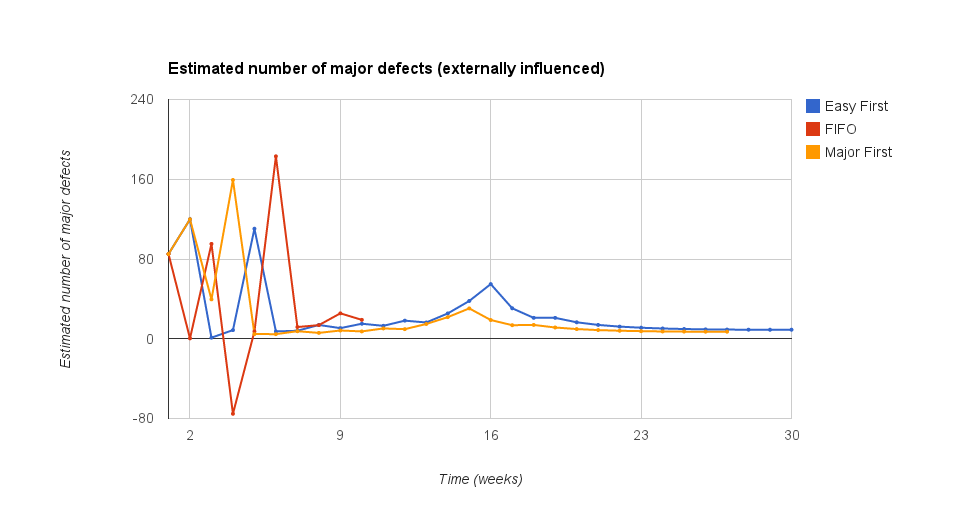
\includegraphics[scale=0.45]{graphs/EstRemMajDef_ex.png}
	\caption{We could not trace this experimental error and thus decided to not use the FIFO strategy
for this measurement.} 
	\label{ex_estremmajdef}
\end{figure}

Other oddities include that the strategies now continue for longer, attempting to finish and
continue fixing defects even though there is nothing new being found or fixed.
They also changed when they stopped due to reassigning the software engineers to testing and fixing
at different times.
Sensible project managers would have stopped testing by now; we have left this in here to showcase
how our system worked.

\pagebreak

We first begin by looking at the external metrics.
As noted earlier, this governs what the client (might!) be thinking about our project and the strategies we have used.

\begin{figure}[ht!]
	\centering
	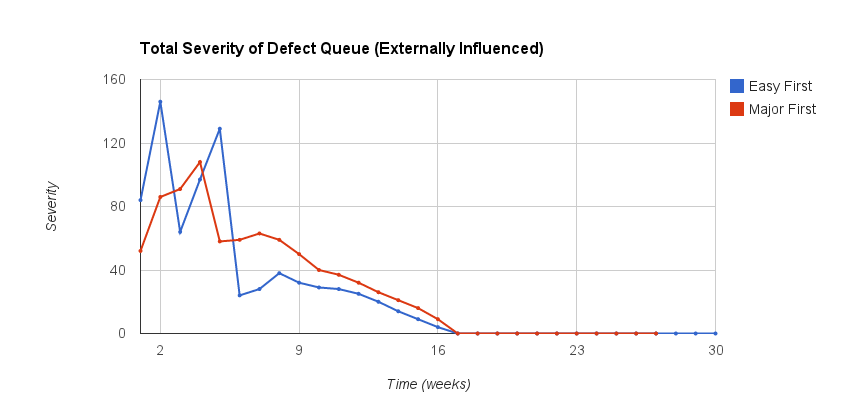
\includegraphics[scale=0.5]{graphs/QueueImpact_ex.png}
	\caption{Notice the large oscillations due to resource reallocation.} 
	\label{ex_qimpact}
\end{figure}

It is interesting that choosing a ``better" strategy is difficult here.
The steadier strategy is to choose major defects first, but the strategy that it is beaten by is to
choose the easier defects first.
The strategy allows spikes in severity levels, however.
We will tentatively claim that here, the easy first strategy is better, despite the sudden surgest
in queue severity.

\pagebreak

What about the average time of major defects in the queue?

\begin{figure}[ht!]
	\centering
	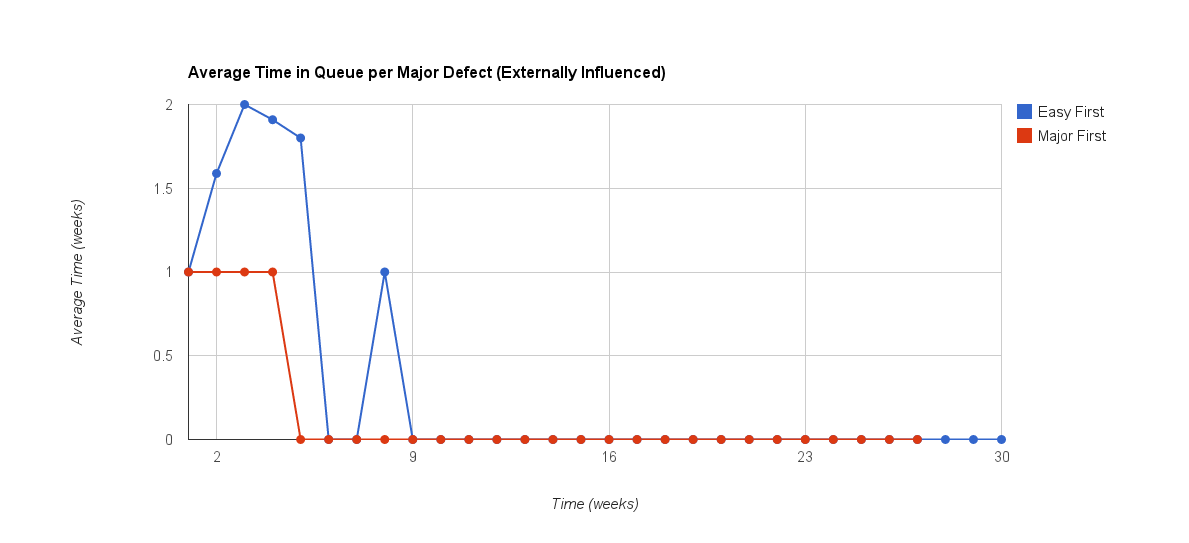
\includegraphics[angle=90,scale=0.4]{graphs/avgMajorQueueTime_ex.png}
	\caption{Overall, high prioritisation of major defects still results in low mean time in queue for
major defects.} 
	\label{ex_avgmajqtime}
\end{figure}

From Figure \ref{ex_avgmajqtime} it is clear that fixing major defects is still the best choice to have a
high performance for average major queue time.

\pagebreak

Next, we briefly examine the find-versus-fixed ratio for major defects.

\begin{figure}[ht!]
	\centering
	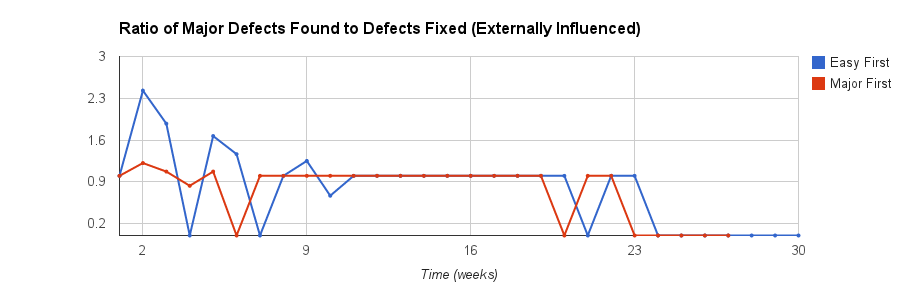
\includegraphics[scale=0.45]{graphs/MajRatioFF_ex.png}
	\caption{Interestingly, very little blowup from the easy strategy --- the resource reallocation is
allowing it to stop the ratio of fixed-found defects from escalating and instead causes it to
oscillate.} 
	\label{ex_majratioff}
\end{figure}

Again we see that the optimal strategy for this metric is to fix major defects first.
However, the differences are much smaller and the strategies are many times on par with each other!
This is quite interesting, when comparing Figure \ref{ex_majratioff} to Figure \ref{majratioff}.

\pagebreak

Next, we examine the internal metrics.
How big is our defect queue size?
Are the resource reallocations causing it to smoothen out a lot?

\begin{figure}[ht!]
	\centering
	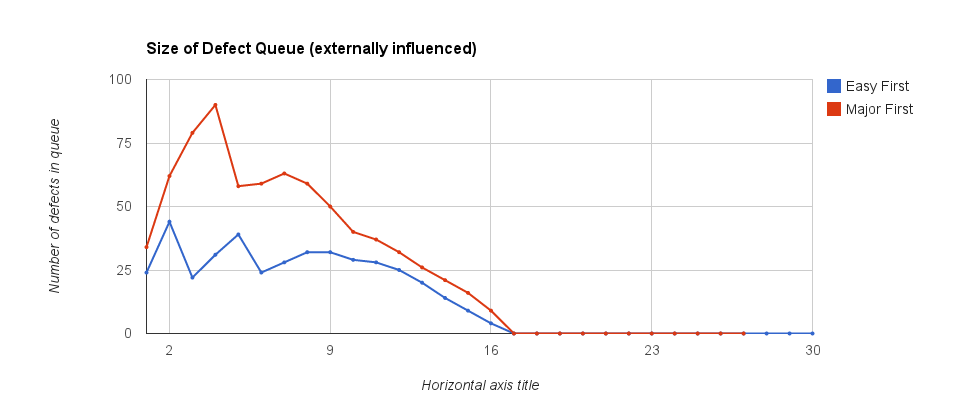
\includegraphics[scale=0.45]{graphs/QueueSz_ex.png}
	\caption{The size of our defects-to-fix queue. Again the optimal choice is to use the easy
strategy.} 
	\label{ex_qsz}
\end{figure}

Figure \ref{ex_qsz} gives what would be the self-evident result --- that prioritising easy defects
yields the best rewards.
There is not as much change here, since severity minimisation does not necessarily entail defect
queue minimisation, as this result shows.\\
\\
We would expect something similar to occur when looking at the average time a defect spends in a
queue, wouldn't we?

\pagebreak

\begin{figure}[ht!]
	\centering
	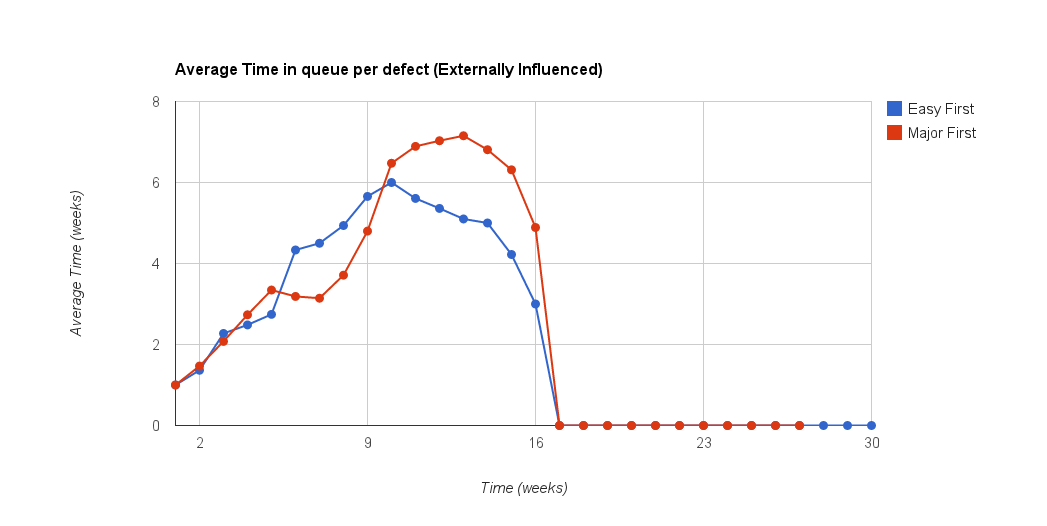
\includegraphics[scale=0.45]{graphs/avgQueueTime_ex.png}
	\caption{This metric seems to be optimally minimised by the easy strategy but fixing major defects
first is very, very close.} 
	\label{ex_avgqtime}
\end{figure}

This seems to be an oscillating reflection of the original results found in Figure
\ref{ex_avgqtime}.
Not a major change, which is a shame as it would have been interesting to see how the previously
optimal strategy, FIFO was affected by resource reallocations.\\
\\
Finally, we showcase the defect ratios for find-versus-fixed.

\pagebreak

\begin{figure}[ht!]
	\centering
	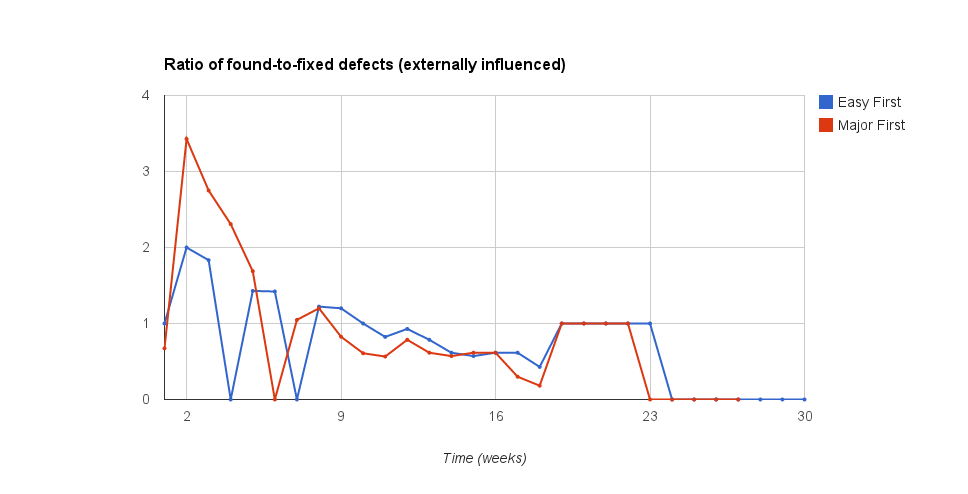
\includegraphics[scale=0.45]{graphs/RatioFF_ex.png}
	\caption{Here, we notice that the optimal choice is to now use the major strategy.} 
	\label{ex_ratioff}
\end{figure}

Figure \ref{ex_ratioff} shows an interesting result! Although major begins poorly, the resource
reallocations have it consistently beating the easy strategy for a large part of the process.
We would tentatively say that major is a better strategy, but that the easy-defects-first strategy
is almost as optimal.\\
\\
We have tabulated our results in a coarse approximation of how ``good" each strategy performed for
each metric.

\begin{table}[ht!]
	\centering
	\begin{tabular}{|c|c|c|}
	\hline
	{\bf Metric} & {\bf Optimal} & {\bf Sub-optimal, but close?} \\ \hline
	{\em Queue Severity} & Easy First & Major First \\ \hline
	{\em Mean time in queue per major defect} & Major First & N/A\\ \hline
	{\em Ratio of Major defects found-to-fixed} & Major First & Easy-first \\ \hline
	Queue Size & Easy First & N/A \\ \hline
	Time in Queue & Easy First & Major First \\ \hline
	Ratio of defects found-to-fixed & Major First & Easy First\\ \hline
	\end{tabular}
	\caption{A summary of our strategies and their performances with different metrics when external
pressure is applied.
External metrics are italicised.
Interestingly, the differences between the strategies have been minimised and they seem to perform
similarly relative to each other.
They all were much more jagged and oscillated a lot due to the sudden resource reallocations.}
	\label{summaryex}
\end{table}

\subsubsection{Internal pressure leading to resource change}

Now, we suppose that if the queue size is too high (that is, there are too many existing defects) then a resource reallocation is required.
It is not a very intelligent decision making system, in that it simply reallocates the resources for
the week and keeps them allocated as such until the queue severity is low again.
Also, the reallocation involves all testers becoming fixers for the week.
We can compare it to a bang-bang controller in embedded systems and robotics.\\
\\
Firstly, we present the estimates of remaining defects.

\begin{figure}[ht!]
	\centering
	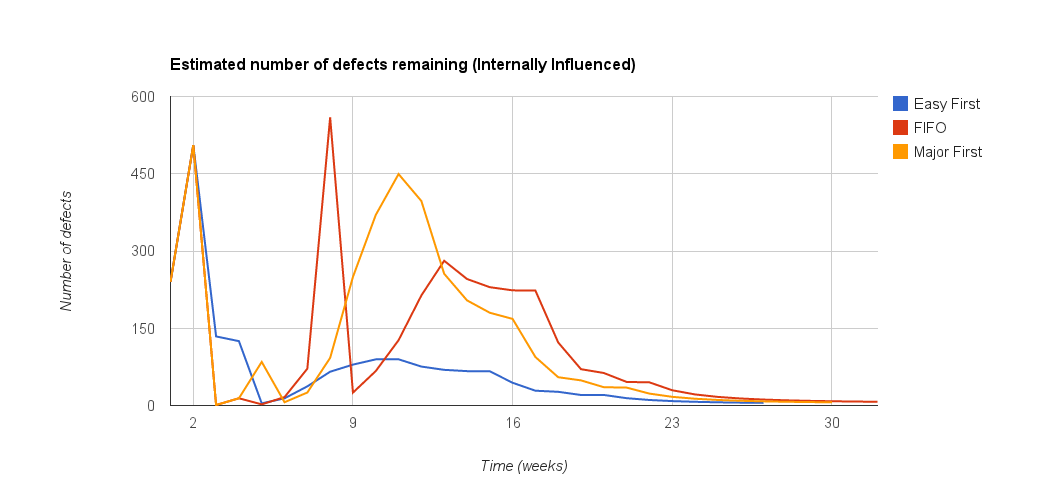
\includegraphics[scale=0.45]{graphs/EstRemDefs_in.png}
	\caption{We note that the resource reallocations again caused high oscillations, except for the
easy strategy.} 
	\label{in_estremdefs}
\end{figure}

Interestingly, the easy strategy appeared to not undergo many resource reallocations or
oscillations.

\pagebreak

A similar result occurs with estimates of remaining major defects.

\begin{figure}[ht!]
	\centering
	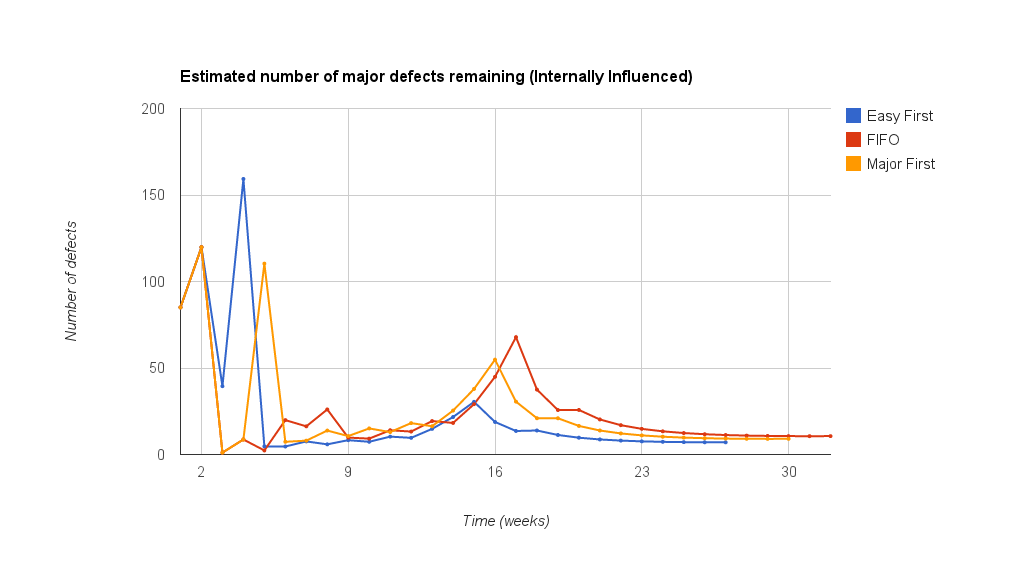
\includegraphics[scale=0.45]{graphs/EstRemMajDef_in.png}
	\caption{This time, it also appears that the FIFO strategy does not have a huge amount of
oscillation.} 
	\label{in_estremmajdef}
\end{figure}

We still have the oddity that the strategies now continue for longer, attempting to finish and
continue fixing defects even though there is nothing new being found or fixed.
Strategies again have different stopping times due to changes for when they stopped due to reassigning the software engineers to testing and fixing
at different times.
Again, a sensible project manager would have stopped testing by now.

\pagebreak

We first begin by looking at the external metrics.
As noted earlier, this governs what the client (might!) be thinking about our project and the strategies we have used.

\begin{figure}[ht!]
	\centering
	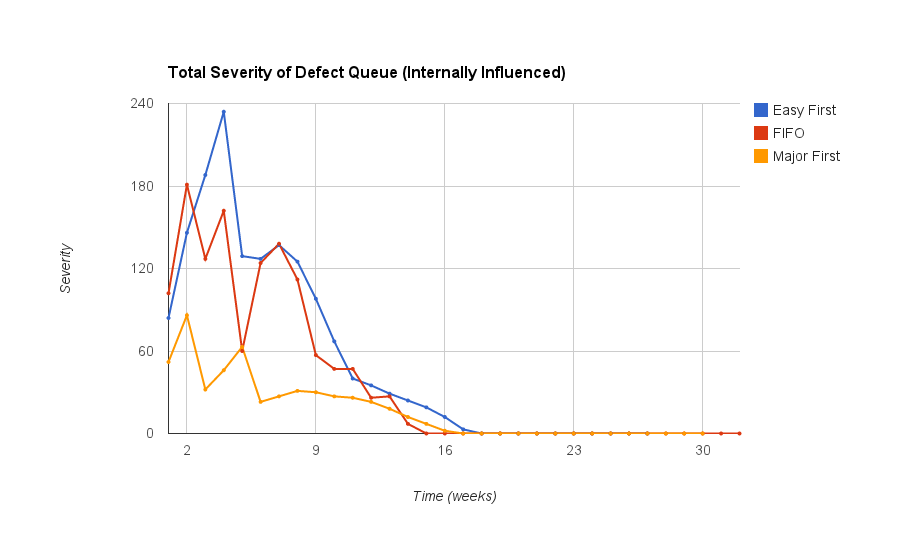
\includegraphics[scale=0.5]{graphs/QueueImpact_in.png}
	\caption{The major-fixes first strategy seems improved by the resource reallocation.}
	\label{in_qimpact}
\end{figure}

It is clear that the major-fixes first strategy is again the best strategy.

\pagebreak

What about the average time of major defects in the queue?

\begin{figure}[ht!]
	\centering
	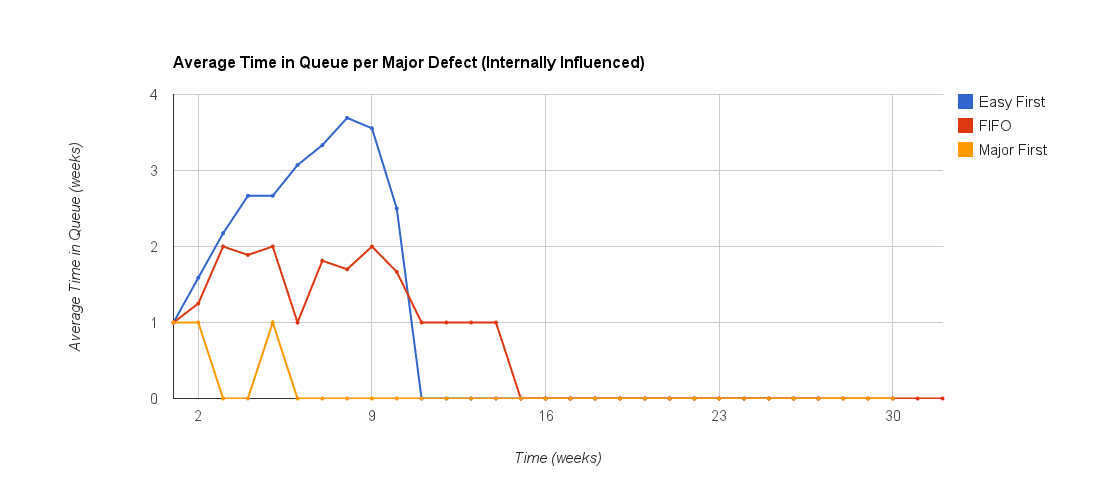
\includegraphics[angle=90,scale=0.4]{graphs/avgMajorQueueTime_in.png}
	\caption{Overall, high prioritisation of major defects still results in low mean time in queue for
major defects.} 
	\label{in_avgmajqtime}
\end{figure}

From Figure \ref{in_avgmajqtime} it is clear that fixing major defects is still the best choice to have a
high performance for average major queue time.

\pagebreak

Next, we briefly examine the find-versus-fixed ratio for major defects.

\begin{figure}[ht!]
	\centering
	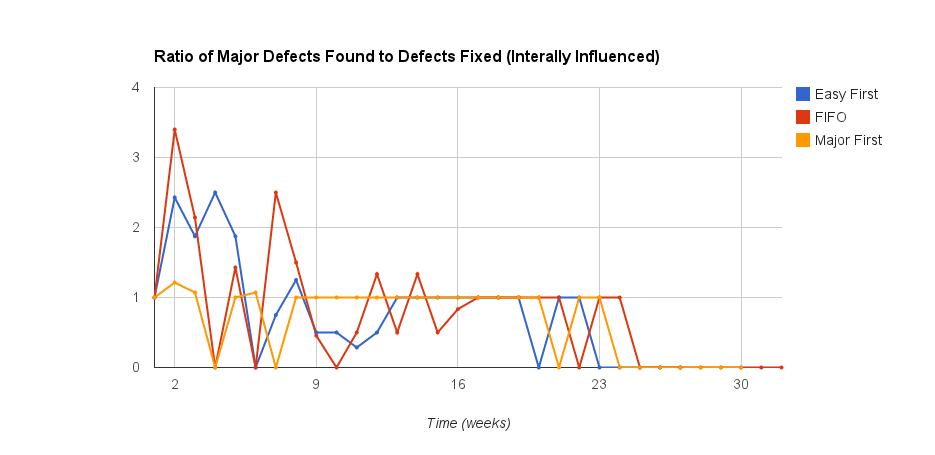
\includegraphics[scale=0.45]{graphs/MajRatioFF_in.png}
	\caption{Interestingly, very little blowup from the easy strategy --- the resource reallocation is
allowing it to stop the ratio of fixed-found defects from escalating and instead causes it to
oscillate.} 
	\label{in_majratioff}
\end{figure}

Again we see that the optimal strategy for this metric is to fix major defects first.
However, the differences are much smaller and the strategies are many times on par with each other!
This is quite interesting, when comparing Figure \ref{in_majratioff} to Figures \ref{majratioff} and
\ref{ex_majratioff}.

\pagebreak

Next, we examine the internal metrics.
How big is our defect queue size?
Are the resource reallocations causing it to smoothen out a lot?

\begin{figure}[ht!]
	\centering
	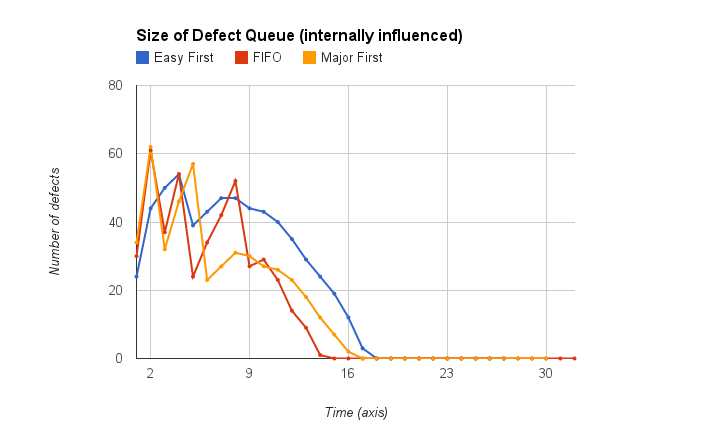
\includegraphics[scale=0.45]{graphs/QueueSz_in.png}
	\caption{The size of our defects-to-fix queue.
An interesting change is that this makes both the FIFO and major-fixes-first strategy better than
the easy-fixes-first strategy.} 
	\label{in_qsz}
\end{figure}

Figure \ref{in_qsz} gives an interesting result --- the resource reallocations have actually
improved the FIFO and major-defects-first strategies.
FIFO is optimal, and major-defects close to being as good in this situation.\\
\\
We would expect something similar to occur when looking at the average time a defect spends in a
queue, wouldn't we?

\pagebreak

\begin{figure}[ht!]
	\centering
	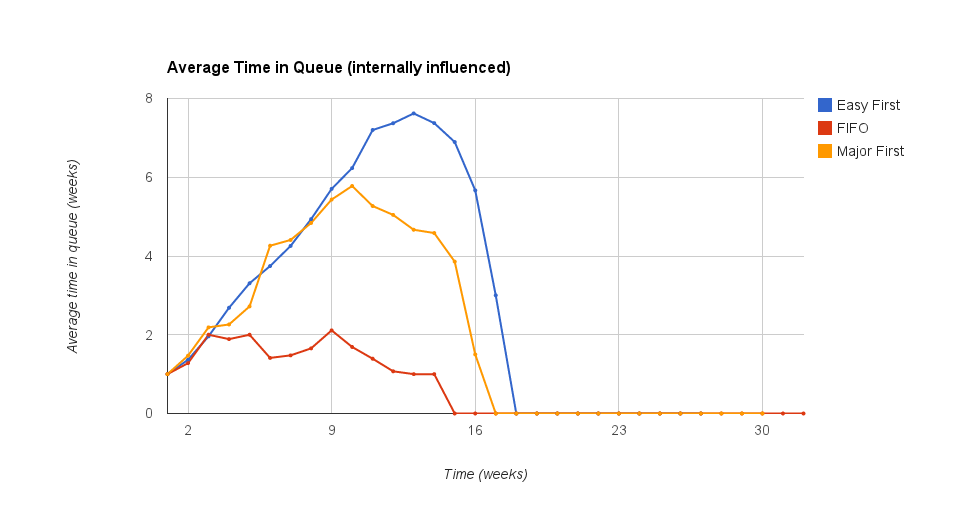
\includegraphics[scale=0.45]{graphs/avgQueueTime_in.png}
	\caption{FIFO is the clear optimal choice here. It already was a queue minimiser and with the
resource reallocation it does even better.} 
	\label{in_avgqtime}
\end{figure}

FIFO is clearly the optimal choice again --- adding the resource reallocation has really made it
minimise time in queue.\\
\\
Finally, we showcase the defect ratios for find-versus-fixed.

\pagebreak

\begin{figure}[ht!]
	\centering
	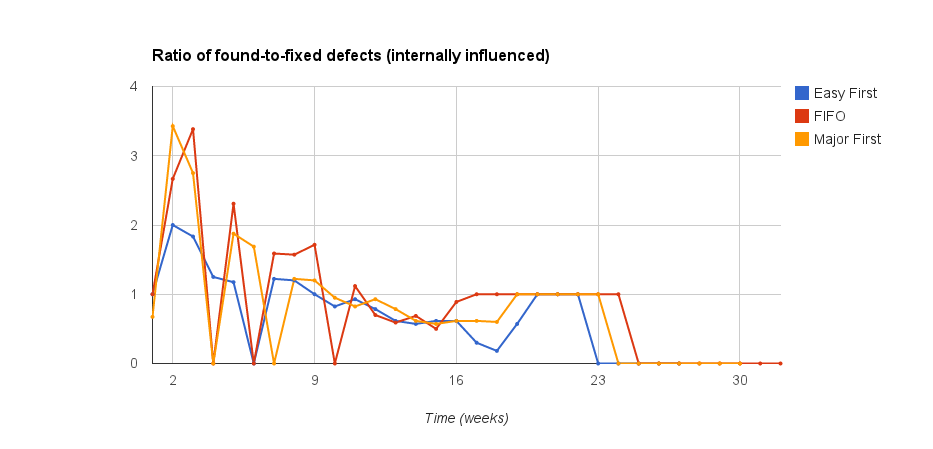
\includegraphics[scale=0.45]{graphs/RatioFF_in.png}
	\caption{The easy-fixes-first is again the best strategy to use in this situation.}
	\label{in_ratioff}
\end{figure}

Surprisingly, there were no changes even after resource reallocations --- the easy-fixes-first was
the best strategy one could use.\\
\\
We have tabulated our results in a coarse approximation of how ``good" each strategy performed for
each metric.

\begin{table}[ht!]
	\centering
	\begin{tabular}{|c|c|c|}
	\hline
	{\bf Metric} & {\bf Optimal} & {\bf Sub-optimal, but close?} \\ \hline
	{\em Queue Severity} & Major First & N/A \\ \hline
	{\em Mean time in queue per major defect} & Major First & N/A\\ \hline
	{\em Ratio of Major defects found-to-fixed} & Major First & Easy-first \\ \hline
	Queue Size & FIFO & N/A \\ \hline
	Time in Queue & FIFO & N/A \\ \hline
	Ratio of defects found-to-fixed & Easy-first & All quite close \\ \hline
	\end{tabular}
	\caption{A summary of our strategies and their performances with different
    metrics wheninternal 
pressure is applied.
External metrics are italicised.
Employing this strategy for resource reallocation (based on queue size) seemed to yield good results, in terms of making
strategies competent against the easy strategy, whilst maintaining properties such as low queue
severity or time of major defect in queue.}
	\label{summaryex}
\end{table}


\section{Analysis} \label{secAnalysis}

With our results in hand, we now return to our seven questions we outlined in
section \ref{secMethod}.
Using our results we will answer each of them and comment on any insights we
have.

\subsection{Question one}

Originally, we wanted to know
\begin{quote}
  To what extent does learning carry over between two software projects of similar
  specifications?
\end{quote}
And, within our experimental framework we translated this to 
\begin{quote}
  What are the differences in $a$ between \PO\ using \LA\ and \PT\ using \LA?
\end{quote}

Our values for $a$ from our best fits for \PO\ using \LA\ and \PT\ using \LA are
shown in Tables \ref{table:P1LA:abc} and \ref{table:P2LA:abc} respectively.
We aggregate them and find that
\begin{itemize}
  \item the average of $a$ in \PO\ using \LA\ is 172.6738 minutes
  \item the standard deviation of our $a$ parameters in \PO\ using \LA\ is 0.23896 
  \item the average of $a$ in \PT\ using \LA\ is 100.0073 minutes
  \item the standard deviation of our $a$ parameters in \PT\ using \LA\ is
  0.068343
\end{itemize}

These low standard deviations suggests that these are very accurate estimates on
the amount of time a student takes to finish off a problem with no information
or knowledge about it.
This is sensible since the $a$ values were all very similar, and each model
should have started off with the same result for the first attempt at finishing
the problems.\\
\\
We note that between the \PO\ in \LA\ and \PT\ in \LA, there was a 72 minute
drop.
This is equivalent to a $42\%$ decrease in the required time to complete the
task, relative to the time taken in \PO\ in \LA.
It seems sensible that knowledge and time taken are inversely correlated.
Our results suggest that after completing a similar task, there is an increase of
$42\%$ in knowledge which is usable for this similar task.
Obviously, this is not entirely true --- there are differences in the tasks we
are using that we have not empirically considered.
Furthermore, we do not have a baseline of solving \PT\ without any prior
knowledge, but this gives an initial estimate on the increase of knowledge.

\subsection{Question two}

Our original question two asked
\begin{quote}
  To what extent does learning carry over between two software projects using
  similar resources?
\end{quote}

Within our experimental framework, this question asked
\begin{quote}
   What are the differences in $a$ between \PO\ using \LA\ and \PO\ using
  \LB?
\end{quote}

Again, we aggregate the $a$ values shown in Table \ref{table:P1LB:abc} and find
that
\begin{itemize}
  \item the average of the $a$ values of \PO\ using \LB\ is 102.9797 minutes
  \item the standard deviation of the $a$ values for \PO\ using \LB\ is 0.655761
\end{itemize}

The drop in $a$ values --- that is, the difference between the mean for \PO\
using \LA\ and \PO\ using \LB\ is very similar to what we found for Question
One.
Indeed, this is a 70 minute decrease, from the initial attempt in \PO\ in \LA\
to the first attempt for \PO\ in \LB.
This is a $40\%$ decrease compared to the $a$ value in \PO\ in \LA, and is quite
comparable to the decrease in the $a$ value in the previous section (\AZ\ of
\PO\ in \LA\ to \AZ\ of \PT\ in \LA).\\
\\
I had a personal suspicion that a language change would have a more significant
increase in knowledge and decrease in time than a change in problem
specification but our results suggest otherwise.
However, I do not think our results are conclusive and might actually support my
suspicions since prior to solving \PT, the students had actually completed \PO\
(a similar problem) problem eight times.
Conversely, when completing \PO\ in \LB\ they had only completed \PO\ four times.
This anomaly in process and experimental methodology suggests that
there is scope for more investigation and that my suspcions should not be
discarded yet.

\subsection{Question three}

Question three originally asks
\begin{quote}
  To what extent does practice enable us to better predict the effort required
  for software?
\end{quote}

This translates to us asking
\begin{quote}
  How well do our models fit the data?
\end{quote}

We want to know whether practice gives us better fits of models --- better fits
will suggest that our models are more useful for later predictions.
To answer this question, we will compare the sum of squares of the three
different datasets.
These are summarised in Tables \ref{table:P1LA:abc:sumsquares},
\ref{table:P1LB:abc:sumsquares} and \ref{table:P2LA:abc:sumsquares}.
We notice that \PO\ using \LA\ gives nonsensical results, and in fact our models
were inappropriate for actually doing much prediction (besides, perhaps $m_3$).
However, in \PT\ using \LA\ and \PO\ using \LB\ we retrieved sensible and useful
results.
\PO\ using \LB\ in particular had very good fits overall, with low sums of least
squares.\\
\\
I believe that this is due to actually practicing more on the same problem ---
we note that after performing the same problem (\PO) multiple times, even in
different languages, gives a more predictable result and is easier to fit a
model to.
Conversely, even though the problem is similar, the learning rate is much more
erratic and difficult to fit when completing \PT, despite using \LA.
This suggests that practicing on the same problem, regardless of language, will give more
consistent and predictable results for modelling purposes, whilst different
problems will cause issues with regards to being able to fit a model.

\subsection{Question four}

Our original question four asks
\begin{quote}
  How does learning differ as we practice on different problems? 
\end{quote}

We translate this, within the framework of our experiment to
\begin{quote}
   How does $b$ change between each of \PO\ in \LA, \PO\ in
   \LB\ and \PT\ in \LA?
\end{quote}

We resummarise all the $b$ results from each dataset, for each model in Table
\ref{table:beees}.

\begin{table}[ht!]
\centering
\begin{tabular}{|c|c|c|c|}
\hline
  & $m_1$ & $m_2$ & $m_3$ \\
\hline
\PO\ in \LA & N/A & N/A & 0.794716 \\
\hline
\PO\ in \LB & 1.05646 & 1.05789 & 1.03095 \\
\hline
\PT\ in \LA & 1.78221 & 1.62075 & 1.39094 \\
\hline
\end{tabular}
\caption{These are the $b$ values from each fit. We omit the unreliable results
for $b$ in $m_1$ and $m_2$ for \PO\ in \LA.}
\label{table:beees}
\end{table}

There is an overall trend of $b$ increasing as the students do more iterations.
We ought to note that the $b$ value increasing makes the curve steeper, and it
reaches its horizontal asymptote (the value for $c$) much more quickly.
This suggests that reinforcement of knowledge through practice increases
learning and is an observable phenomena.\\
\\
An interesting question to ask is if the learning itself is asymptotic.
How much practice could we do before we would not increase learning anymore?
Figure \ref{fig:BvalueFit} is a graph showing the means of the $b$ values and
the overall trend polynomial trend.

\begin{figure}[ht!]
\centering
\FIXME
\caption{The $b$-values after aggregation between each dataset.}
\label{fig:Bvaluefit}
\end{figure}

I think that we do not have enough data to make a conclusive comment about this,
but it is important to note that at present, the learning value apparently
is unbounded, and furthermore increases at an unbounded rate (by taking the
derivative of the equation of best fit).
This seems nonsensical to me, and I would suggest doing further analyses beyond
this rudimentary inspection to determine how learning changes and how learning
itself is affected between each iteration.

\section{Conclusion}

% Every research paper should answer the following questions:
% 
% \begin{itemize}
% \item What did you do?
% \item Why did you do it?
% \item What happened?
% \item What do the results mean?
% \item What is your work good for?
% \end{itemize}
% 
% Make sure that your conclusion leaves the reader with the answers
% to these questions clearly in mind.
% 

% appendices

\appendix

\section{Simulation Framework} \label{simframe}

%\chapter{Project Proposal}

In many software development articles, quality is a vague, implicitly defined
concept.
Denning, Buthmann and Soni each discuss quality and the prevention of defects without explicitly
defining what quality {\em is} \cite{Soni:2010:DP, Buthmann:2010:CQ,
	Denning:1992:ESQ:129617.384272}.
What is common to many definitions of ``quality" is the need to minimise the number of defects and to
meet and exceed customer expectations.
I am particularly interested in the first of these characteristics.\\
\\
The minimisation of defects is itself a subjective criteria that relies on the fitness of a design
with respect to reliability, robustness and maintainability.
I will not consider these within my project and will instead focus on tools and techniques that are
(hopefully) largely independent of previous stages of software development and thus as general as
possible.

\section{Primary Goals}

I would like to examine the current state of the art in detecting and reducing defects in code.
This includes, but is not limited to the investigation of
\begin{itemize}
	\item the effectiveness of defect detection techniques like structured walkthroughs and code
	review
	\item whether employing revision control has influenced software development practice, and if so
	how (especially in the open source scene)
	\item how processes like the Personal Software Process (PSP) and Team Software Process (TSP) are
	affecting software development
\end{itemize}

\section{Secondary Goals}

My project will have auxillary, extension goals, which complement but are not essential to its
completion.
I will outline these three goals.
\begin{itemize}
	\item small-scale testing of some processes and tools to discuss their effectiveness
	\item research into the uptake of, and employment of techniques and tools within industry and the
	open source software scene
	\item the construction of, and discussion about the effectiveness of a personal developer process
	will minimise defects on a per-patch basis
\end{itemize}


\bibliographystyle{ieeetr}
\bibliography{assTwo}

\end{document}
